\documentclass[12pt, letterpaper]{article}
\usepackage[utf8]{inputenc}
\usepackage[russian]{babel}
\usepackage{amsmath}
\usepackage{xfrac}
\usepackage{arcs}
\usepackage[document]{ragged2e}


\title{Устный Зачёт по Геометрии}
\author{Скорбенко Егор}
\date{Апрель 2018}

\begin{document}
\maketitle
\tableofcontents

\section {Дайте определение угла между векторами, скалярного произведения векторов. Сформулируйте условие перпендикулярности. Докажите теорему о вычислении скалярного произведения векторов через их координаты. Выведите формулу для вычисления угла между векторами.}
\subsection{Определения}
Угол между векторами- угол между направлениями этих векторов.\\
Скалярным произведением двух векторов называется произведение их длин на косинус угла между ними. \\
Условие перпендикулярности- скалярное произведенеие ненулевых векторов равно нулю тогда и только тогда, когда эти векторы перпендикулярны. \\
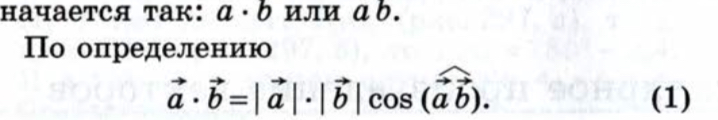
\includegraphics[scale=0.3]{photo.jpg} \\
\subsection {Теорема о вычислении скалярного произведения векторов через их координаты.}
В прямоугольной системе координат скалярное произведение векторов $\vec{a}$ и $\vec{b}$ выражается формулой \\
\begin{center}
$\vec{a}*\vec{b}={x_1}{x_2}+{y_1}{y_2}$
\end{center}
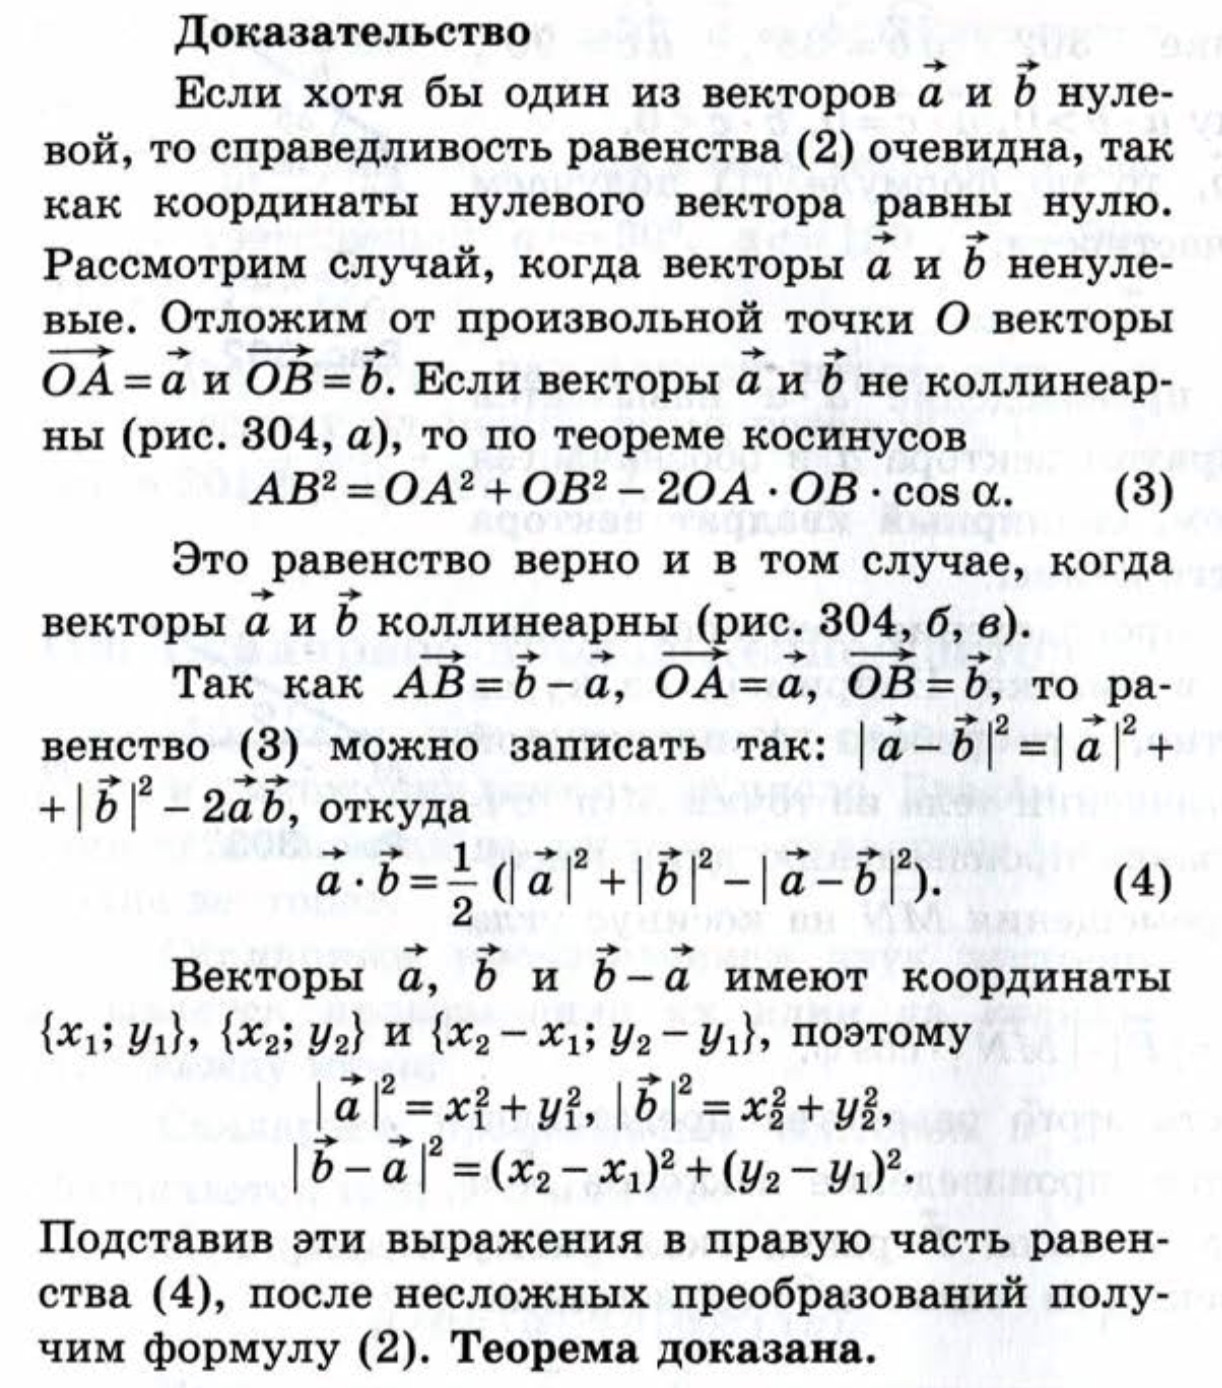
\includegraphics[scale=0.3]{photo2.jpg} \\
\subsection {Вывод формулы для вычисления угла между векторами.}
Углом между двумя векторами, отложенными от одной точки, называется кратчайший угол, на который нужно повернуть один из векторов вокруг своего начала до положения сонаправленности с другим вектором. \\
Косинус угла между векторами равен скалярному произведению векторов, деленному на произведение модулей векторов. \\
\begin{center}
$ \cos a =\dfrac{\overline{a}*\overline{b}}{\dfrac{}{\left|a\right|}*{\left|b\right|}} $ \\
\end{center}


\section {Сформулируйте и докажите свойства скалярного произведения векторов.}
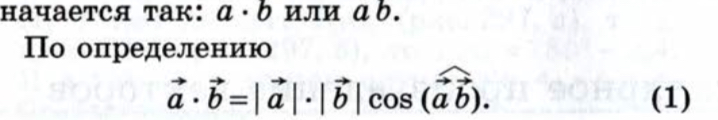
\includegraphics[scale=0.3]{photo.jpg} \\
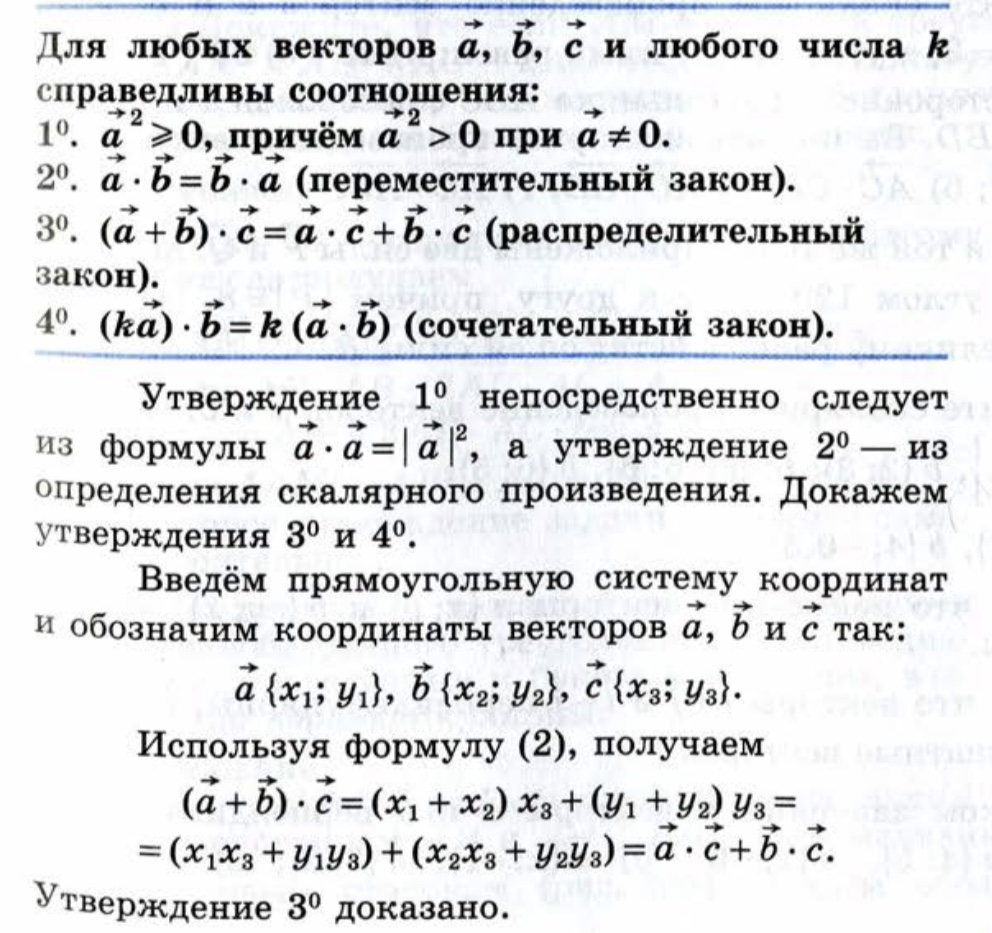
\includegraphics[scale=0.3]{photo1.jpg} \\
\includegraphics[scale=0.3]{photo3.jpg} \\

\section {Дайте определение правильного многоугольника. Докажите, что около любого правильного многоугольника можно описать окружность.}
\subsection{Определения}
\textbf{Правильным многоугольником} называется выпуклый многоугльник, у которого все углы равны и все стороны равны. \\
Окружность называется описанной, если все вершины многоугольника лежат на данной окружности. \\
Около любого правильного многоугольника можно описать окружность, и притом только одну. \\
\subsection{Доказательство}
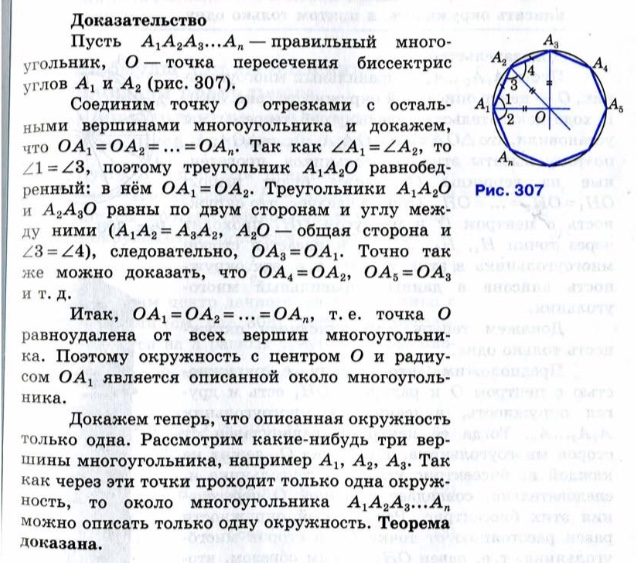
\includegraphics[scale=0.3]{photo4.jpg}

\section {Дайте определение правильного многоугольника. Докажите, что в любой правильный многоугольник можно вписать окружность.}
\subsection{Определения}
\textbf{Правильным многоугольником} называется выпуклый многоугльник, у которого все углы равны и все стороны равны. \\
Окружность называется вписанной, если все стороны многоугольника касаются данной окружности. \\
В любой правильный многоугольник можно вписать окружность, и притом только одну. \\
\subsection{Доказательство}
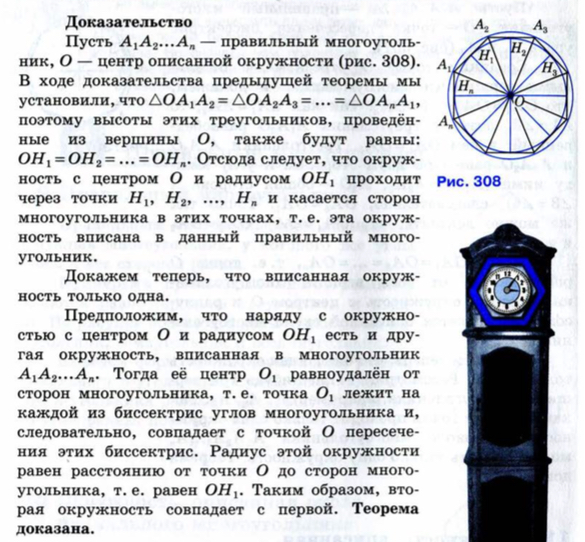
\includegraphics[scale=0.3]{photo5.jpg}

\section {Выведите формулы для вычисления элементов правильного многоугольника (длина стороны, радиус вписанной окружности,  площадь) через радиус описанной окружности.}
Докажем, что $S=\dfrac{1}{2}Pr$. \\
$S=\dfrac{1}{2}Pr=n*\dfrac{1}{2}*a*r=\dfrac{1}{2}*(n*a)r$ \\ 
\textbf{ЧТД.} \\
Далее:
$ a_n=2R*\sin \dfrac{180^{\circ}}{n} $ \\
$ r=R*\cos \dfrac{180^{\circ}}{n}$ \\
$ \angle A_1 = \dfrac{\alpha_n}{2}=\dfrac{n-2}{2n}*180^{\circ}=90^{\circ}-\dfrac{180^{\circ}}{n}. $ \\
$ a_n=2*A_1*H_1 $ \\
$ r=O*H_1 $ \\

\section {Выведите формулы для вычисления элементов правильного многоугольника (радиус описанной окружности, радиус вписанной окружности, площадь) через длину стороны.}
????????????

\section {Выведите формулы для вычисления радиуса описанной окружности и радиуса вписанной окружности в произвольном треугольнике}
???????

\section {Дайте определения градуса и радиана. Выразите приближенное значение одного радиаиа в градусах. Выведите формулы для нахождения длины дуги через ее градусную меру и радианную.}
\subsection{Определения}
Градус- единица измерения дуг и углов, равная 1/360 окружности. \\
Радиан- угол, соответствующий дуге, длина которой равна её радиусу. \\
1 Градус $\approx$ 0.0175 Радиан \\
\subsection{Формула через радианную меру}
$ l=\dfrac{\pi R}{180} n $ \\
\subsection{Формула через градусную меру}
Градус -> радиан и аналогично пункту 2. \\ 


\section {Выведите формулы для нахождения площадей частей круга. }

\section {Сформулируйте свойства и признаки равнобедренной трапеции. Сформулируйте и допишите свойство равнобедренной трапеции с перпендикулярными диагоналями.}

\section {Дайте определение движения. сформулируйте общие свойства. Перечислите виды движений и их свойства.}
\subsection{Определения}
Движение плоскости- отображерние плоскости на себя, сохраняющее расстояния. \\
Центральная симметрия плоскости также является движением. \\
\subsection{Общие свойства}

\subsection{Виды движений}
1. Симметрия осевая \\
2. Симметрия центральная \\
3. Симметрия зеркальная \\
4. Симметрия скользащая \\
5. Параллельный перенос \\
6. Поворот \\




\section {Докажите теорему о произведении отрезков пересекающихся хорд окружности. Докажите теорему о произведении отрезков секущей и квадрате касательной, проведенных из одной точки.}

\subsection{Теорема о произведении отрезков пересекающихся хорд окружности}
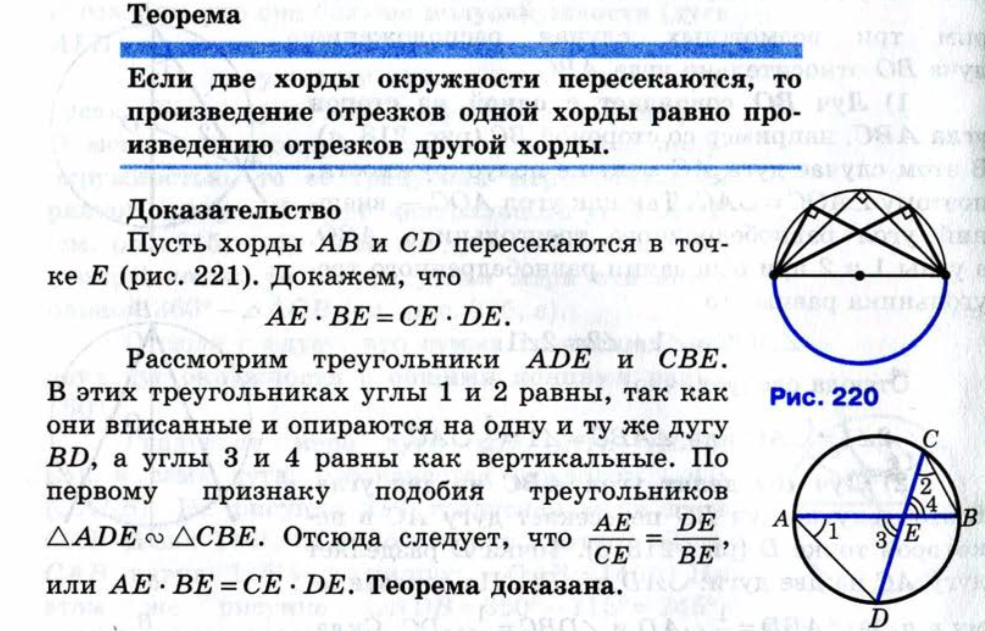
\includegraphics[scale=0.3]{photo10.jpg}
\subsection{Теорема о произведении отрезков секущей и квадрате касательной, проведенных из одной точки.}
\textbf{$CB*AC=CD^2$ \\}
$\Delta ACD $ и $ \Delta DCB $ \\
$ \angle ACD = \angle DCB $ \\ 
$ \angle ADC  = \dfrac{1}{2} \overarc{AD} $ \\
$ \angle ABD  = \dfrac{1}{2} \overarc{AD} $ \\
$ \angle ABD  = \angle ADC $ \\
$ \Delta ACD $ подобен $ \Delta DCB $. \\


\section {Сформулируйте и докажите теорему о величине угла между касательной и хордой.}
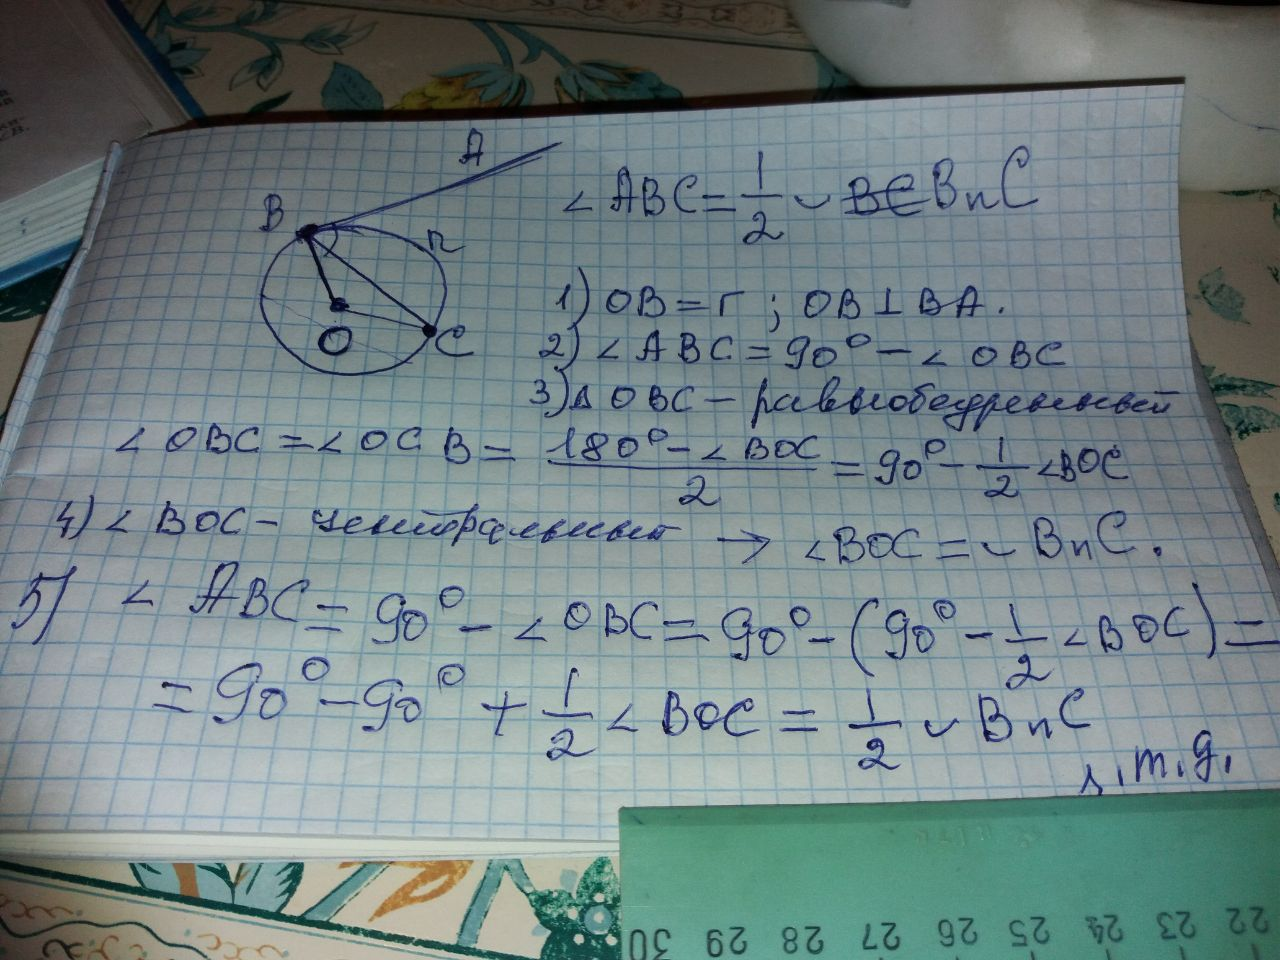
\includegraphics[scale=0.3]{asset-2.png} \\

\section {Сформулируйте и докажите теоремы о величине углов между пересекающимися хордами, между секущими.}
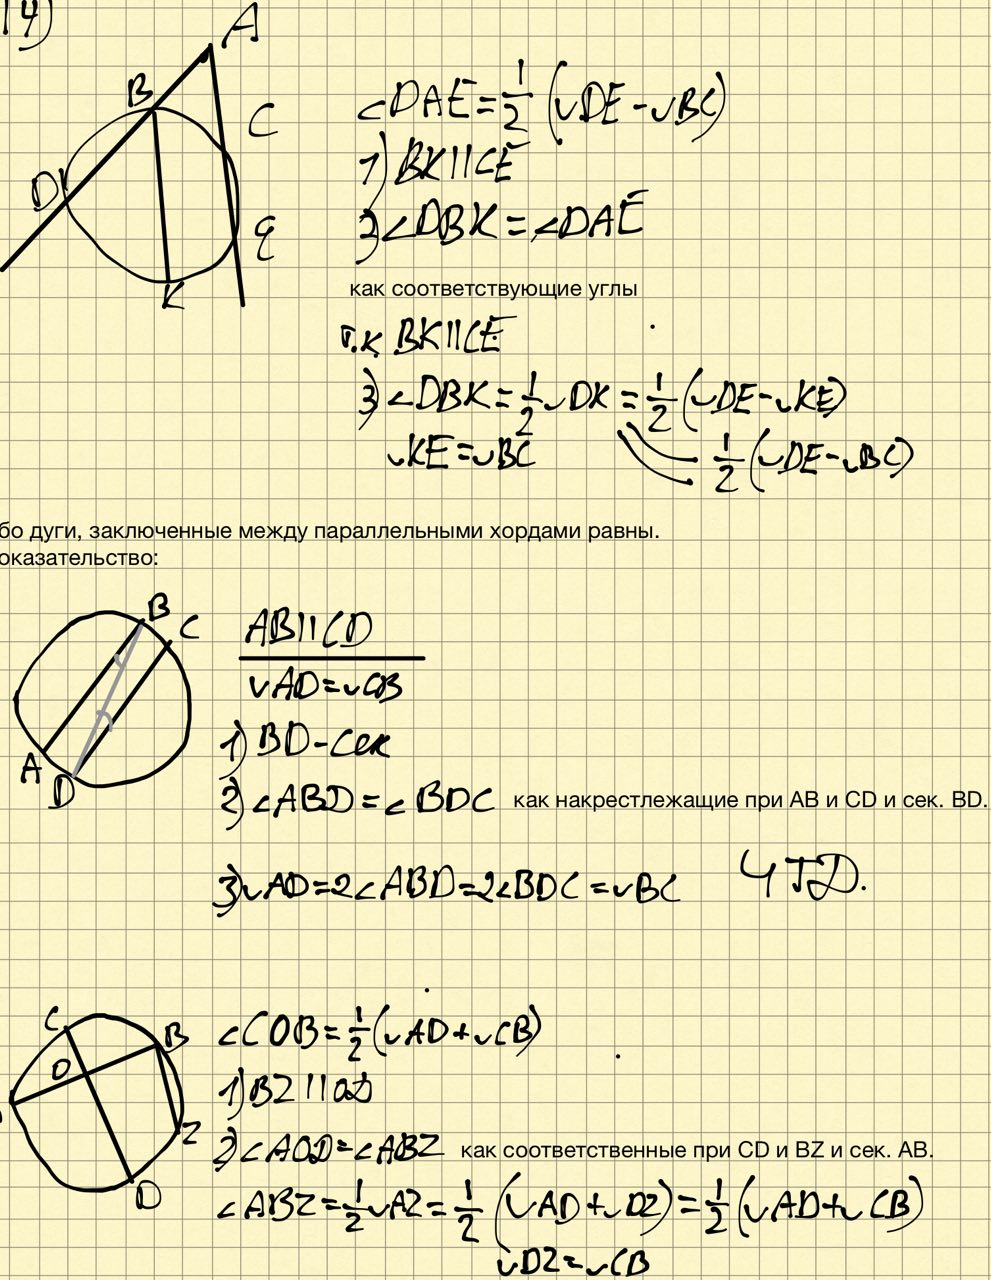
\includegraphics[scale=0.3]{asset.jpg} \\


\section {Сформулируйте и докажите теорему о сумме квадратов диагоналей параллелограмма.}
в предыдущем зачете

\section {Сформулируйте и докажите свойство диагоналей параллелограмма и формулу для вычисления длины медианы.}
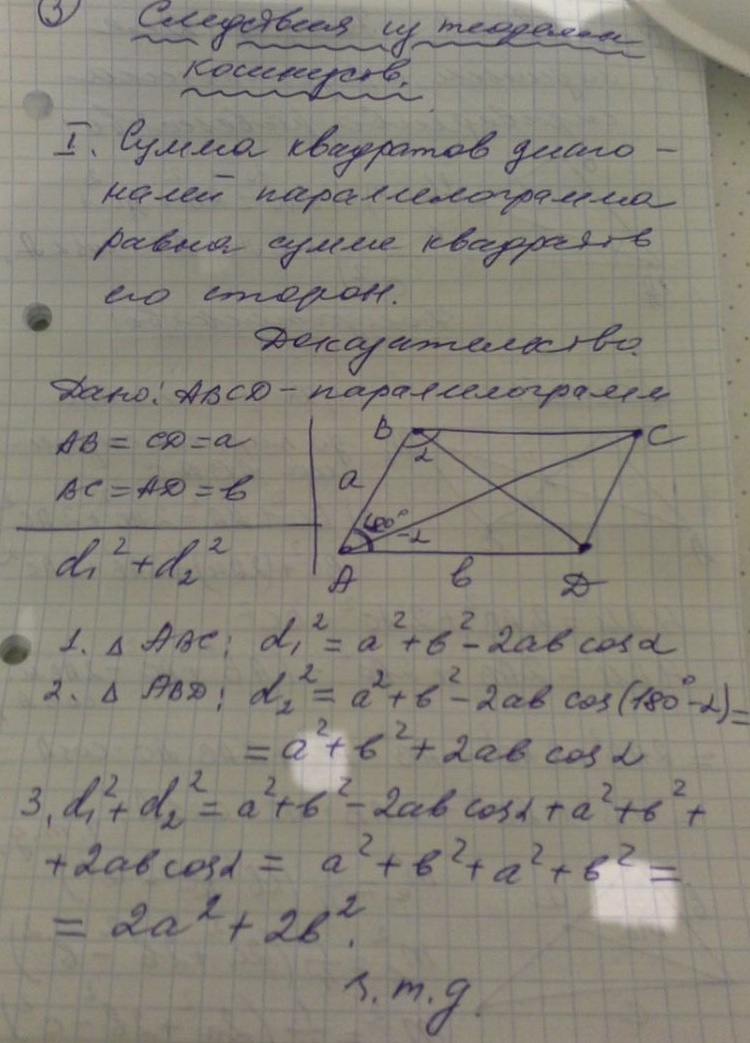
\includegraphics[scale=0.3]{bilet16.jpg} \\
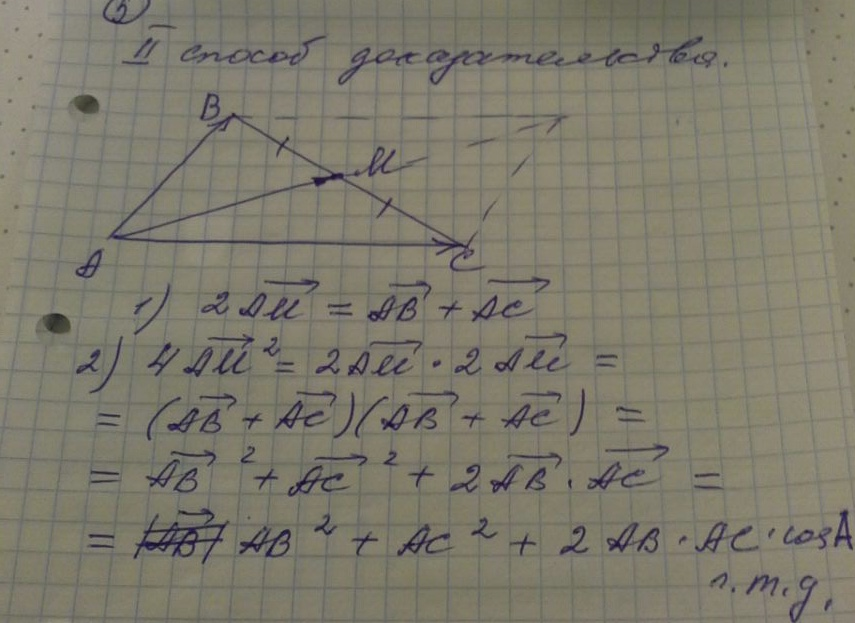
\includegraphics[scale=0.3]{bilet16-1.jpg} \\
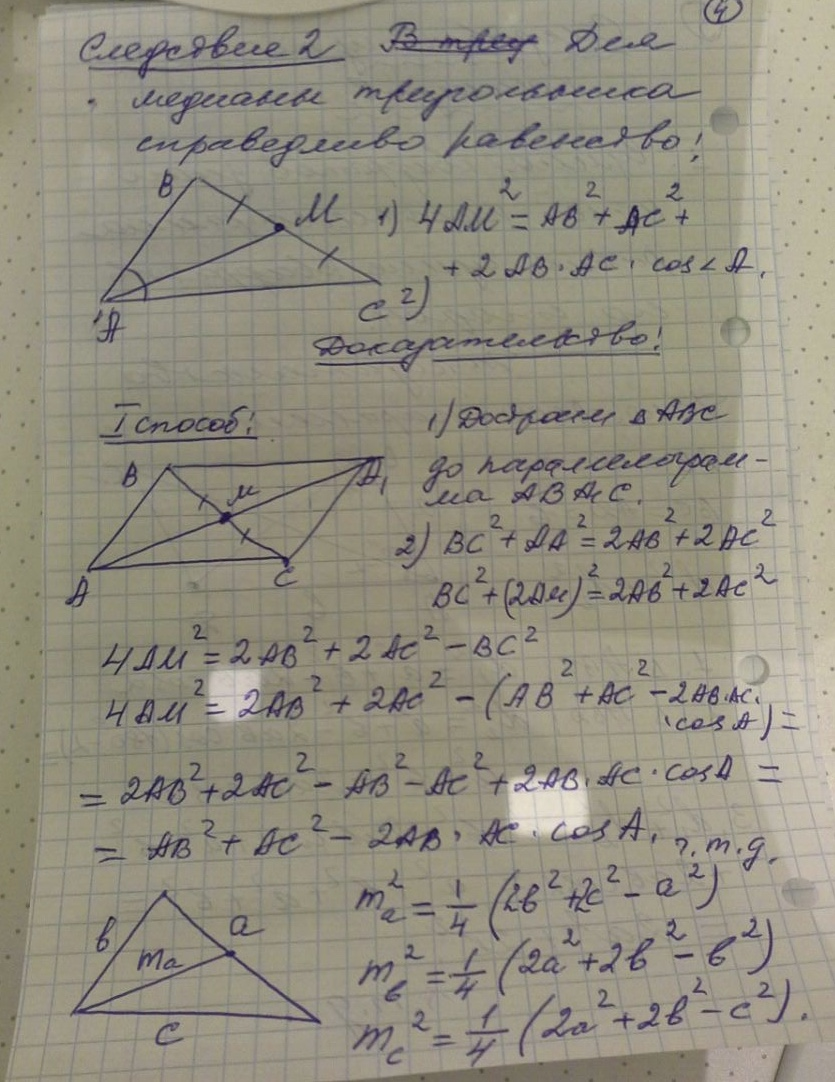
\includegraphics[scale=0.3]{bilet16-2.jpg} \\

\section {Сформулируйте признаки подобия треугольников. Докажите один из них по выбору.}
\subsection{Определения}
Два треугольника называются \textbf{подобными}, если их углы соответственно равны и стороны одного треугольника пропорциональны сходственным сторонам другого треугольника. \\
1. Если два угла одного треугольника соответственно равны двум углам другого, то такие треугольники подобны. \\
2. 2 стороны пропорциональны + угол равен \\
3. 3 стороны пропорциональны \\

\begin{center}
$ \dfrac{AB}{A_1 B_1} = \dfrac{BC}{B_1 C_1} = K $ \\ 
\end{center}

\subsection{Доказательство}
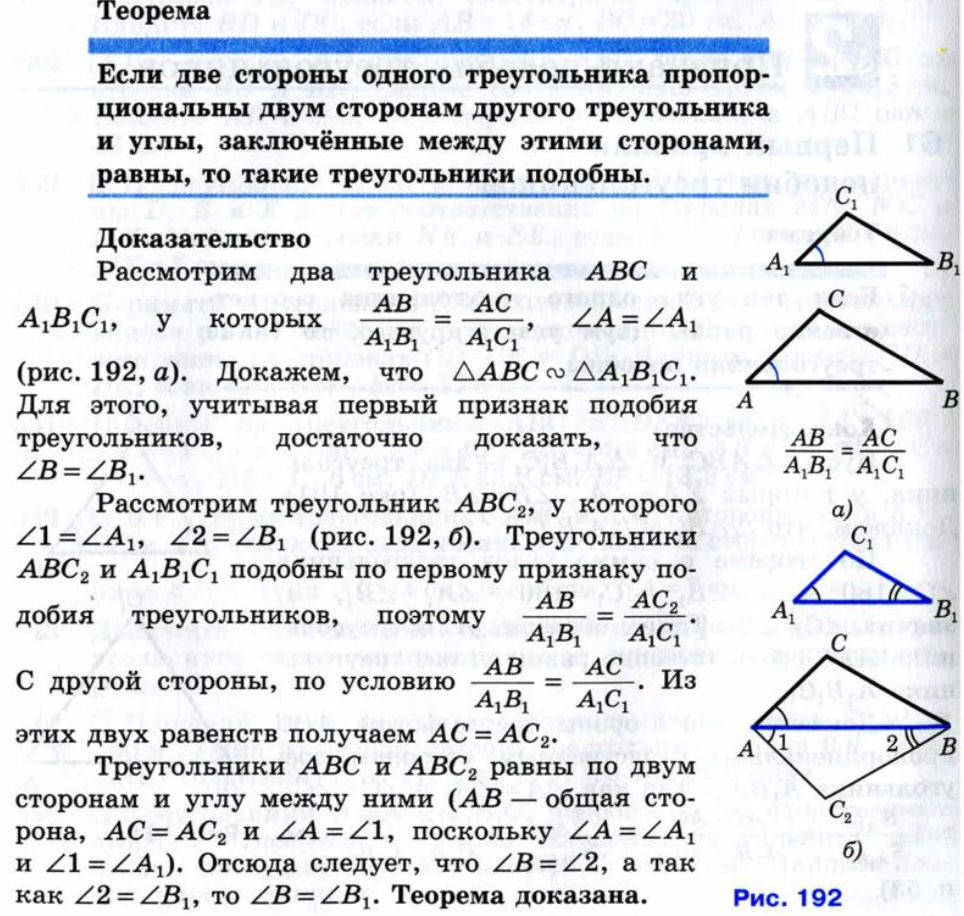
\includegraphics[scale=0.3]{photo8.jpg} \\

\section {Сформулируйте и докажите обобщенную теорему синусов.}
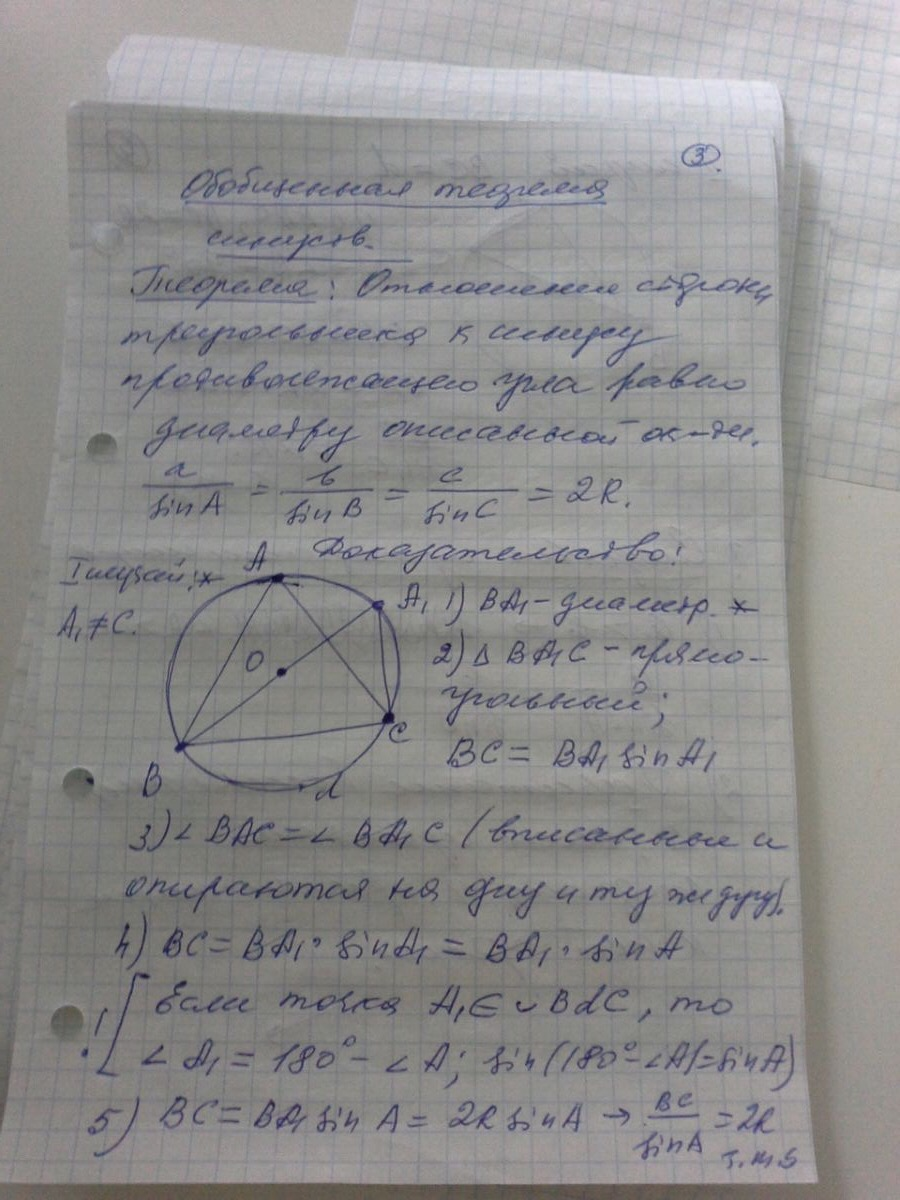
\includegraphics[scale=0.3]{photo6.jpg} \\
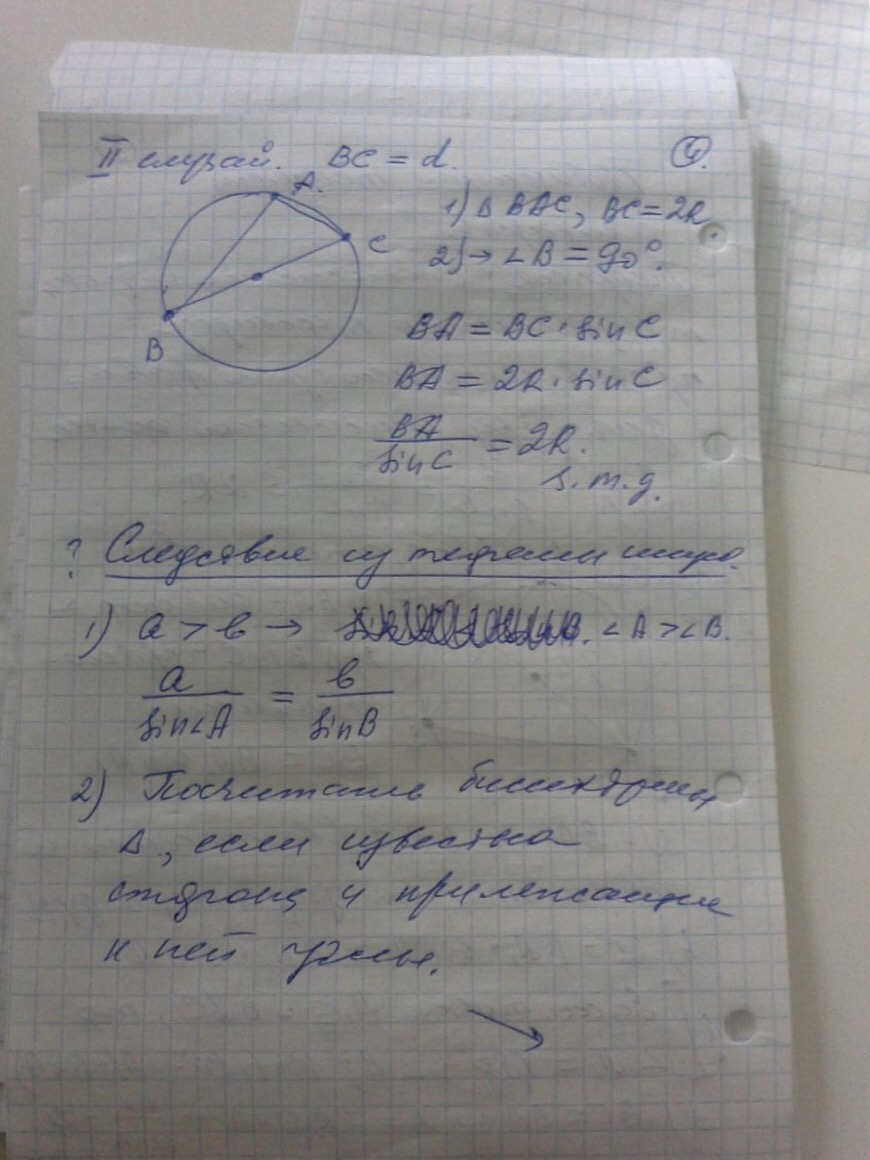
\includegraphics[scale=0.3]{photo7.jpg} \\

\section {Выведите формулы для нахождения пропорциональных отрезков в прямоугольном треугольнике. Выведите формулу для нахождения высоты прямоугольного треугольника через его стороны.}
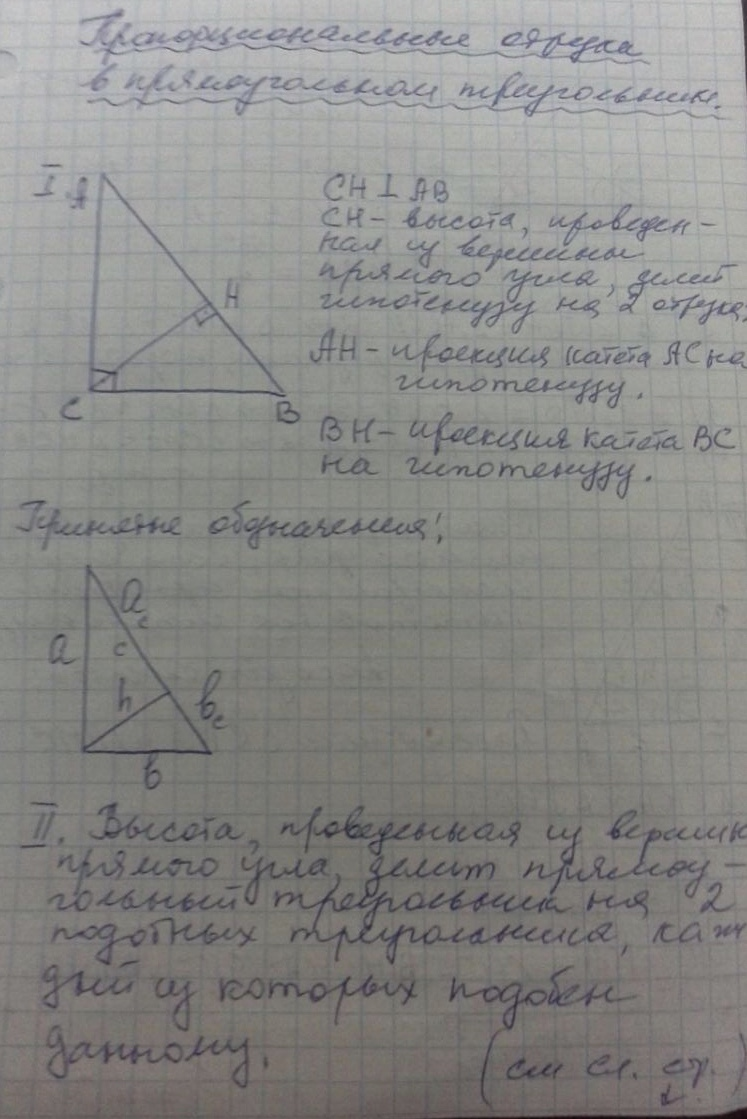
\includegraphics[scale=0.3]{solve19.jpg} \\
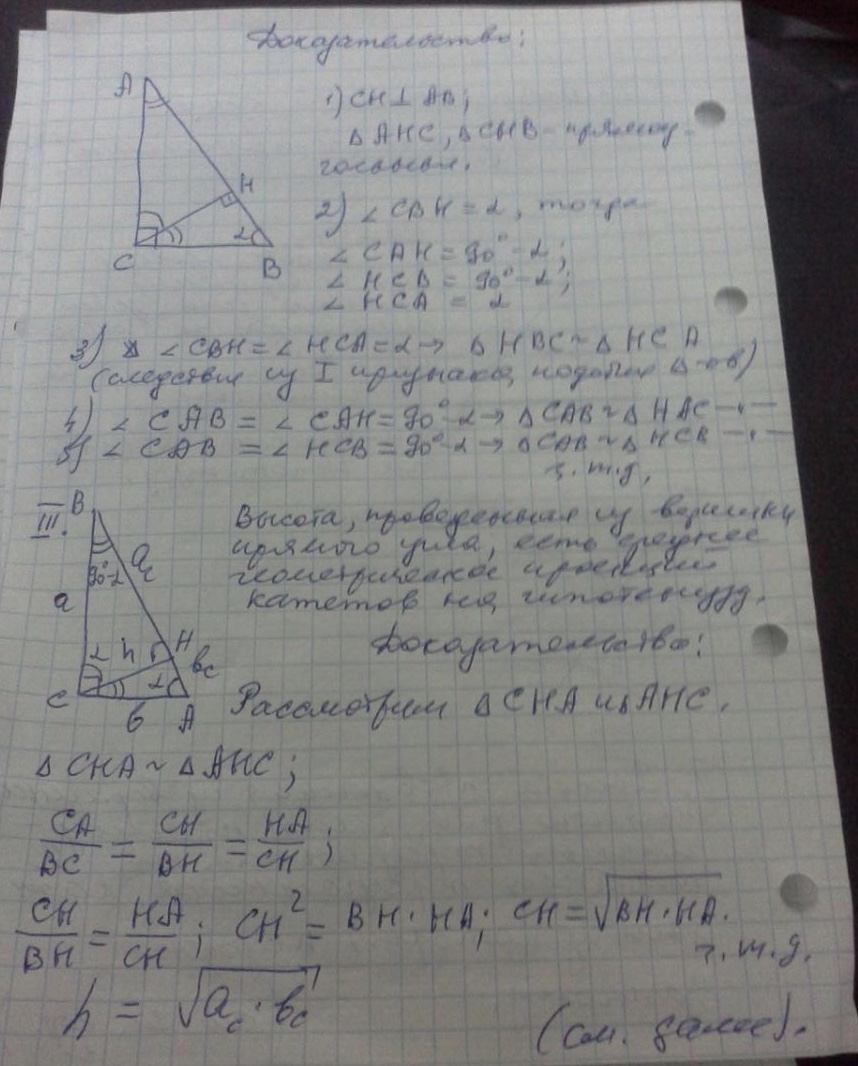
\includegraphics[scale=0.3]{solve19-1.jpg} \\
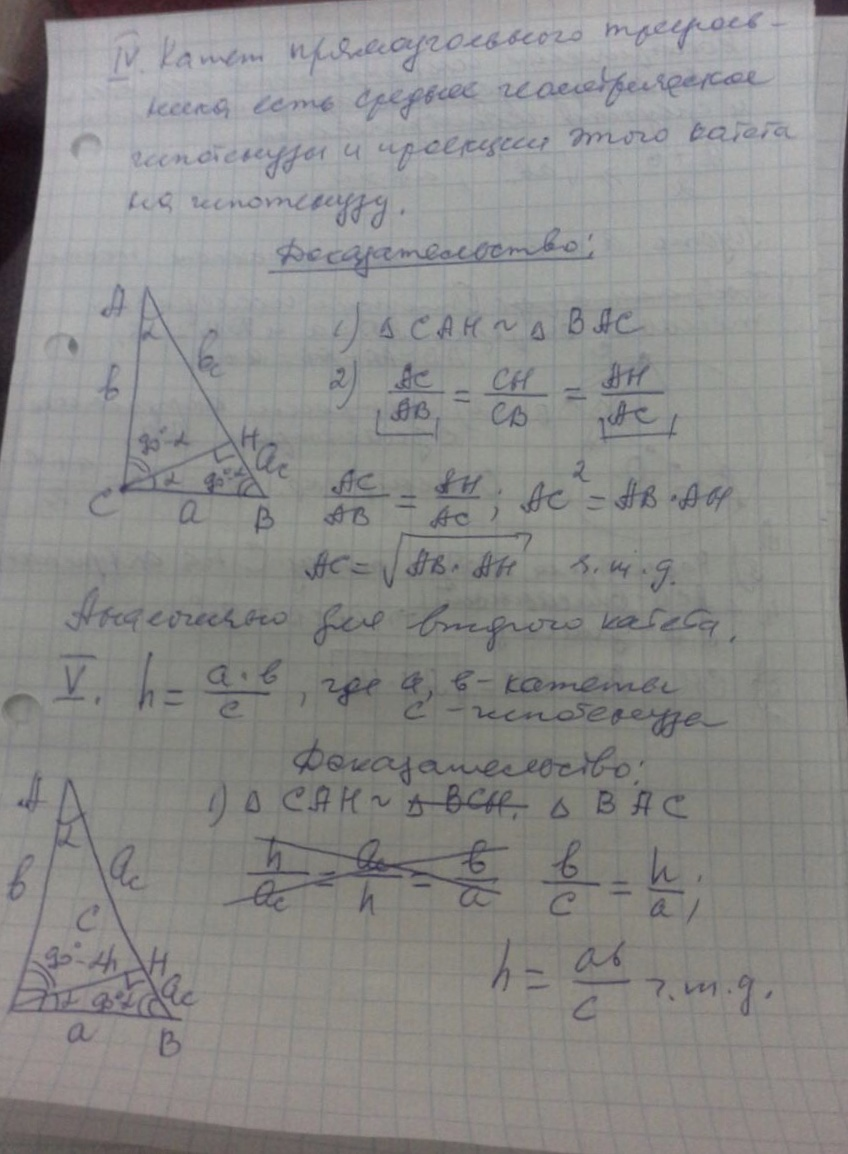
\includegraphics[scale=0.3]{solve19-2.jpg} \\

\section {Выведите формулы для нахождения площади треугольника. (Не менее 4)}
\subsection {Стандартная}
$S=\dfrac{1}{2}ah $ \\
\textbf{Доказательство:} достроим до параллелограмма ABCD,\\
$\Delta ABC = \Delta DCB = \dfrac{1}{2}ABCD. $ \\

\subsection {Формула Герона}
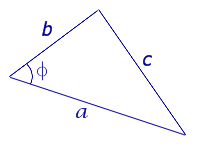
\includegraphics[scale=1]{asset.png} \\
$S=\sqrt{(p(p-a)(p-b)(p-c))}$ \\
$p=\dfrac{P}{2}=\dfrac{a+b+c}{2}$ \\
\textbf{Доказательство:} \\
\begin{flushleft}
$S=\dfrac{1}{2}absin\phi$ => $S^2=\dfrac{1}{4}a^2b^2sin^2\phi=\dfrac{1}{4}a^2b^2(1-cos^2\phi).$ \\
$c^2=a^2+b^2-2abcos\phi$ => $cos\phi=\dfrac{a^2b^2-c^2}{2ab}=cos^2\phi$\\
$S^2=\dfrac{1}{4}a^2b^2(1-cos^2\phi)= $ \\
$ \dfrac{1}{4}a^2b^2(1-(\dfrac{a^2+b^2-c^2}{2ab})^2)=$ \\
$ \dfrac{1}{16}(4a^2b^2-(a^2+b^2-c^2)^2)= $ \\
$ \dfrac{1}{16}((a+b)^2-c^2)(c^2-(a-b)^2)= $ \\
$ \dfrac{1}{16}(a+b+c)(a+b-c)(c+a-b)(c-a+b)= $ \\
$ \dfrac{1}{16}(a+b+c)(a+b+c-2c)(c+a+b-2b)(a+b+c-2a)= $ \\ 
$ \dfrac{1}{16}2p(2p-2c)(2p-2b)(2p-2a)= p(p-c)(p-b)(p-a)$ \\
\end{flushleft}
\textbf{$ S=\sqrt{(p(p-a)(p-b)(p-c))} $ ЧТД.}

\subsection {Полупериметр и вписанная окружность}
$S=\dfrac{1}{2}Pr$ \\
\textbf{Доказательство:} \\
\begin{flushleft}
$S=\dfrac{1}{2}Pr=n*\dfrac{1}{2}*a*r=\dfrac{1}{2}*(n*a)r$ \\
\end{flushleft}

\subsection {Формула через синус}
$S=\dfrac{1}{2}ab*sin\alpha $ \\
\textbf{Доказательство:} \\
\begin{flushleft}
$h_a=b*\sin \alpha $ \\
$S=\dfrac{1}{2} a*h_a= \dfrac{1}{2}ab*\sin \alpha $ \\
\end{flushleft}


\section {Выведите формулу площади произвольного четырехугольника и формулу площади дельтоида.}
\subsection{Определения}
\textbf{Дельтоид}- четырехугольник, в котором есть две пары равных смежных сторон. \\

\subsection{Формула площади произвольного четырехугольника}

$S=\dfrac{1}{2}BD*AC*\sin{\phi}$\\
$S_\Delta=\dfrac{1}{2}l*m*\sin{}$\\
$S_0 = S_1 + S_2 + S_3 + S_4 = \dfrac{1}{2}AO*OB * \sin{\phi} + \dfrac{1}{2}BO*OC*\sin{180-\phi} + \dfrac{1}{2}OC*OD*\sin{\phi} + \dfrac{1}{2}OD*OA*\sin{180-\phi}$
$=\dfrac{1}{2}\sin{\phi}(AO*OB+OB*OC+OC*OD+OD*OA)=\dfrac{1}{2}\sin{\phi}(OB(AO+OC)+OD(OC+OA))=\dfrac{1}{2}\sin{\phi}(OB+OD)(AO+OC)=\dfrac{1}{2}\sin{\phi}BD*AC$ \\
\textit{ЧТД.}\\
\textbf{Cинусы смежных углов равны.}

\subsection{Формула площади дельтоида}
1. BD перпендикулярен AC \\
2. $ S=\dfrac{1}{2} d_1 d_2 \sin{\phi} $ \textbf{но} $\angle \phi = 90$ => $\sin{\phi}=1$ \\


\section {Сформулируйте и докажите теорему о центре окружности, вписанной в треугольник. Сформулируйте и докажите теорему о центре окружности, описанной около треугольника.}
п77, п78
\section {Сформулируйте и докажите свойство биссектрисы треугольника.}
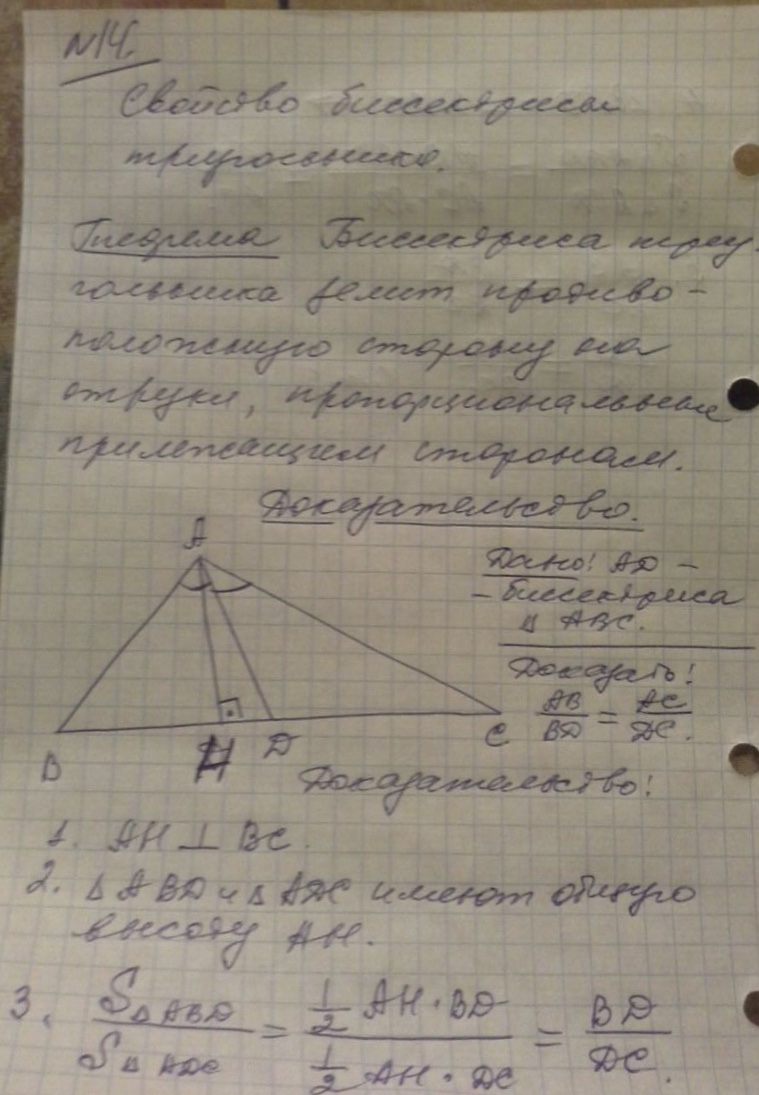
\includegraphics[scale=0.3]{solve14.jpg} \\
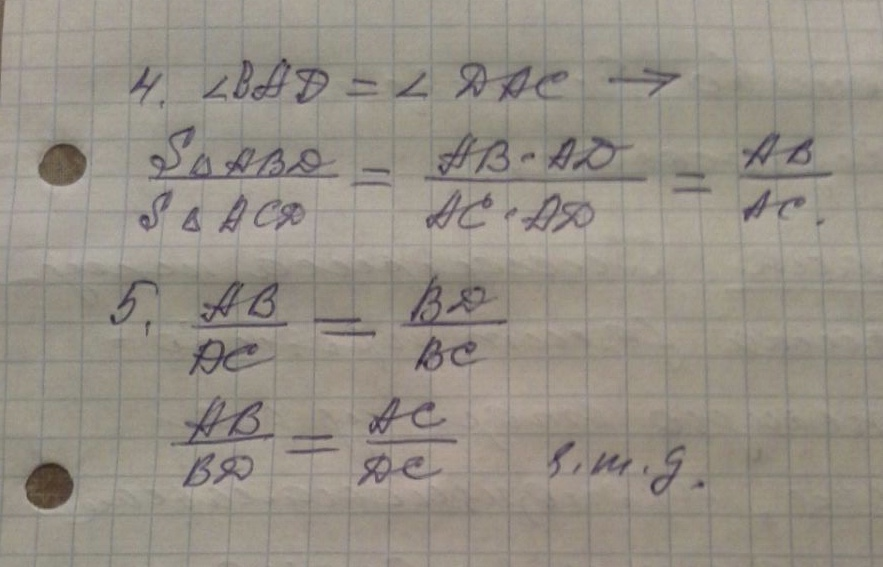
\includegraphics[scale=0.3]{solve14-1.jpg} \\
\section {Сформулируйте и докажите свойство биссектрис параллелограмма.}
\section {Сформулируйте и докажите три свойства равнобедренной трапеции}
\section {Сформулируйте и докажите признаки прямоугольного треугольника. (Теорема, обратная теореме Пифагора и соотношение медианы и стороны, к которой она приведена.}
\subsection{Признаки}
1. Теорема, обратная теореме Пифагора. \\
2. Теорема о соотношении медианы и стороны, к которой она проведена. \\

\subsection{Теорема, обратная теореме Пифагора.}
Дано: $\Delta$ABC, $c^2=a^2+b^2$ \\
1. Построим прямоугольный треугольник $A_1 B_1 C_1$, такой что $\angle C_1 = 90 $, $b_1=b$, $a_1=a$ \\
2. $\angle C_1=90; A_1 B_1^2 = A_1 C_1^2+C_1 B_1^2 = b^2+a^2$, однако по условию:\\
3. $b^2+a^2=c_1^2 = A_1 B_1^2$; так как $A_1 B_1>0, c>0$, то: \\
4. $A_1 B_1 = C$ \\
=> \\
5. $AC = A_1 C_1 $ по построению \\
5. $BC = B_1 C_1 $ по построению \\
5. $AB = A_1 B_1 $ по пунктам выше, то есть \\
6. $\Delta ABC = \Delta A_1 B_1 C_1 $ => $\angle C = \angle C_1 = 90 $ \\

\subsection{Теорема соотношения медианы и стороны, к которой она приведена?}
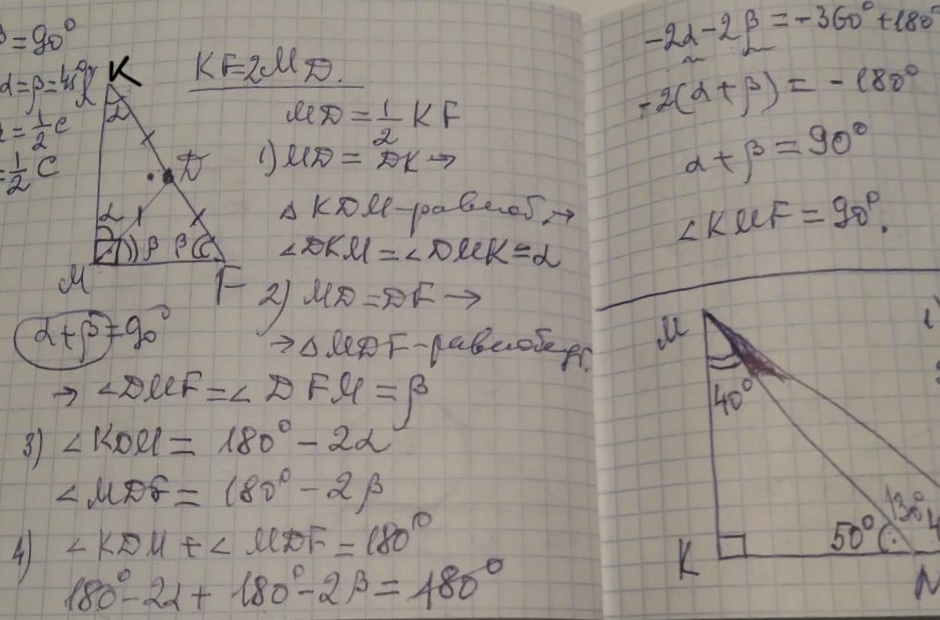
\includegraphics[scale=0.3]{photo9.jpg} \\

\section {Выведите формулы для нахождения радиусов вписанной и описанной окружностей через стороны правильных треугольника, квадрата и шестиугольника.}
ФОФ
\section {Дайте определение вписанного угла. Сформулируйте и докажите теорему о величине вписанного угла.}
в предыдущем зачете декабре
\section {Сформулируйте и докажите свойство медиан в произвольном треугольнике.}
фофо

\section {Сформулируйте теорему Чевы. Сформулируйте и докажите теорему Менелая.}
\subsection{Чевы}
Если AL, BM и CK пересекаются в одной точке, то: \\
$\dfrac{AK}{KB}*\dfrac{BL}{LC}*\dfrac{CM}{MA}=1$\\
\subsection{Менелая}
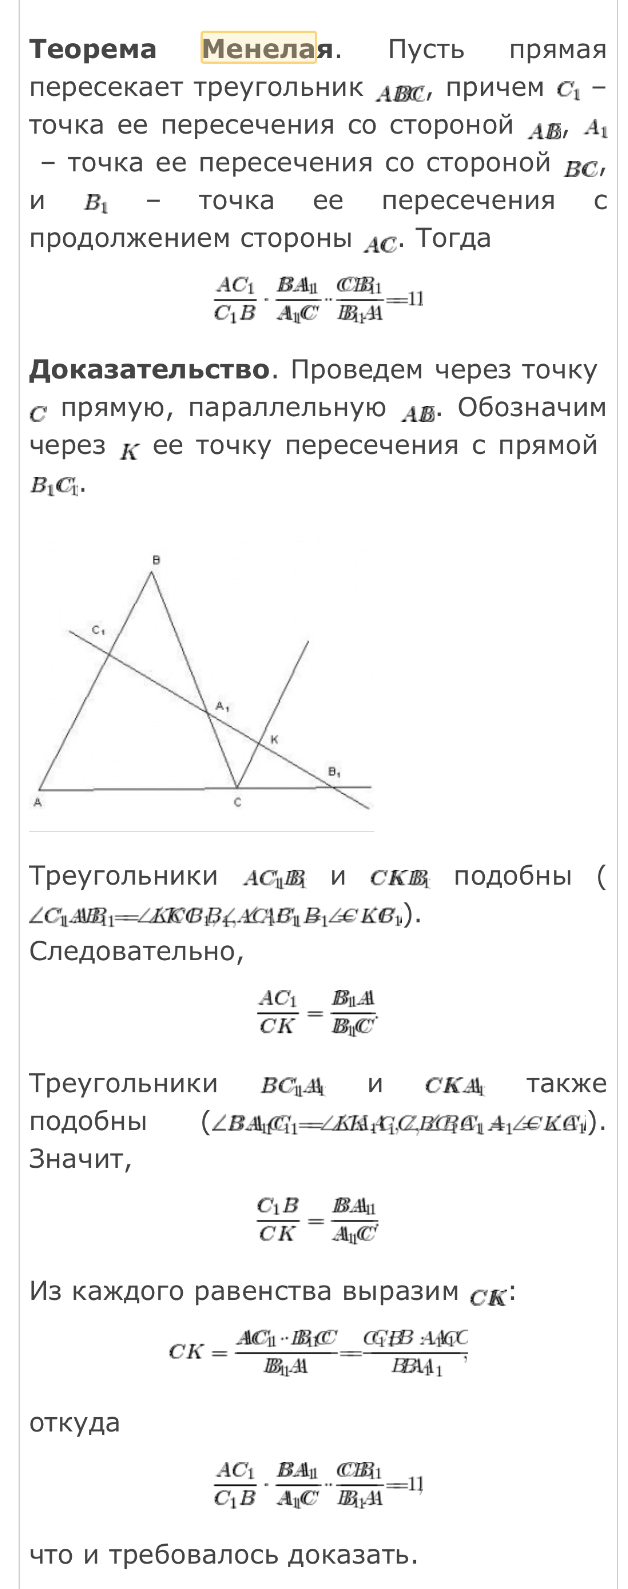
\includegraphics[scale=0.3]{solve30.jpg}\\
\section {Сформулируйте и докажите свойства площадей треугольников с равными высотами, треугольников с равным углом и треугольников справными основаниями.}
\section {Сформулируйте и докажите свойства вписанного и описанного четырехугольника.}
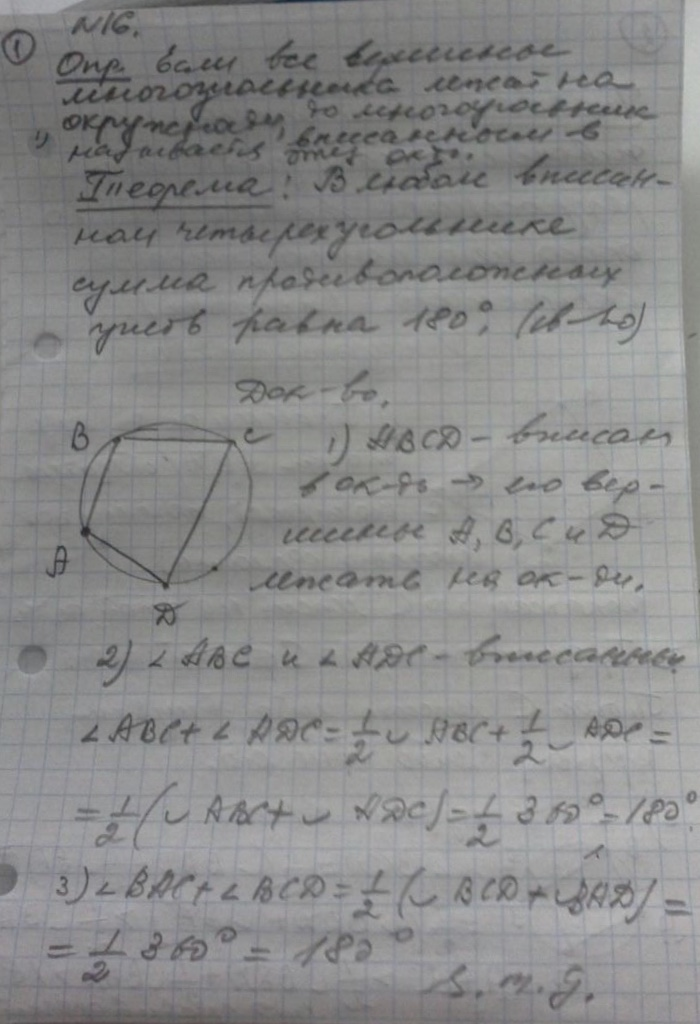
\includegraphics[scale=0.3]{solve16.jpg} \\
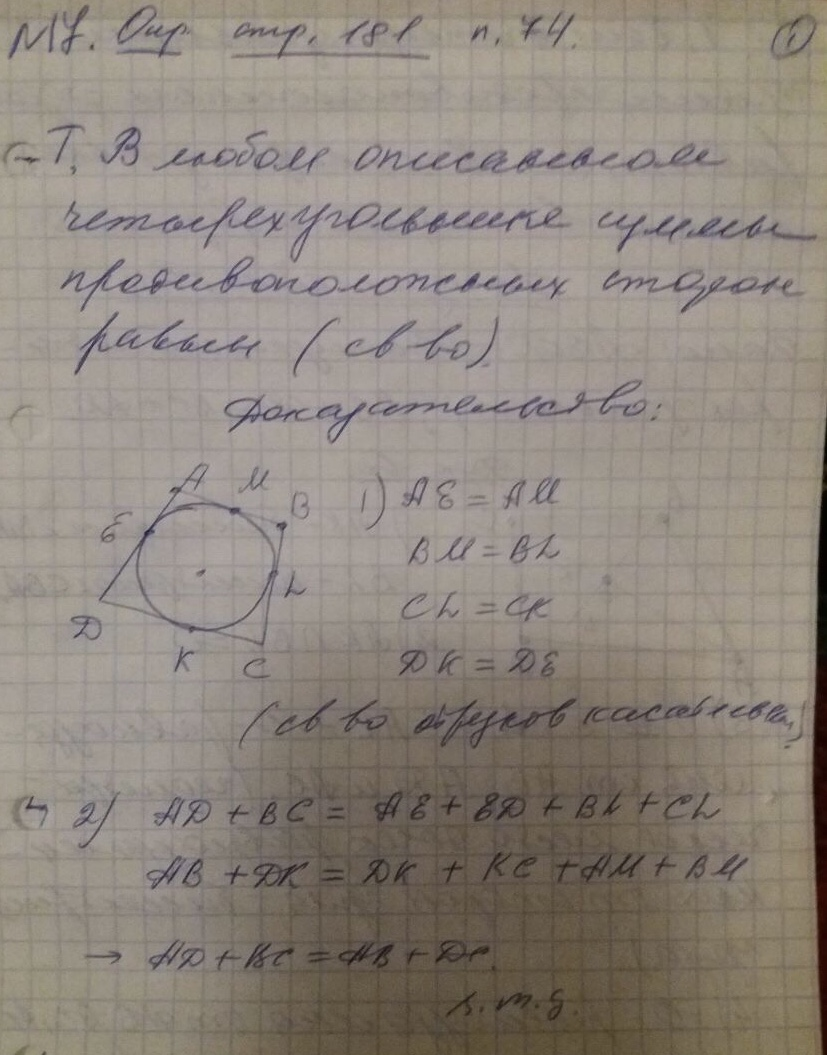
\includegraphics[scale=0.3]{solve17.jpg} \\
\section {Найдите радиус вписанной и описанной окружностей прямоугольного треугольника.}
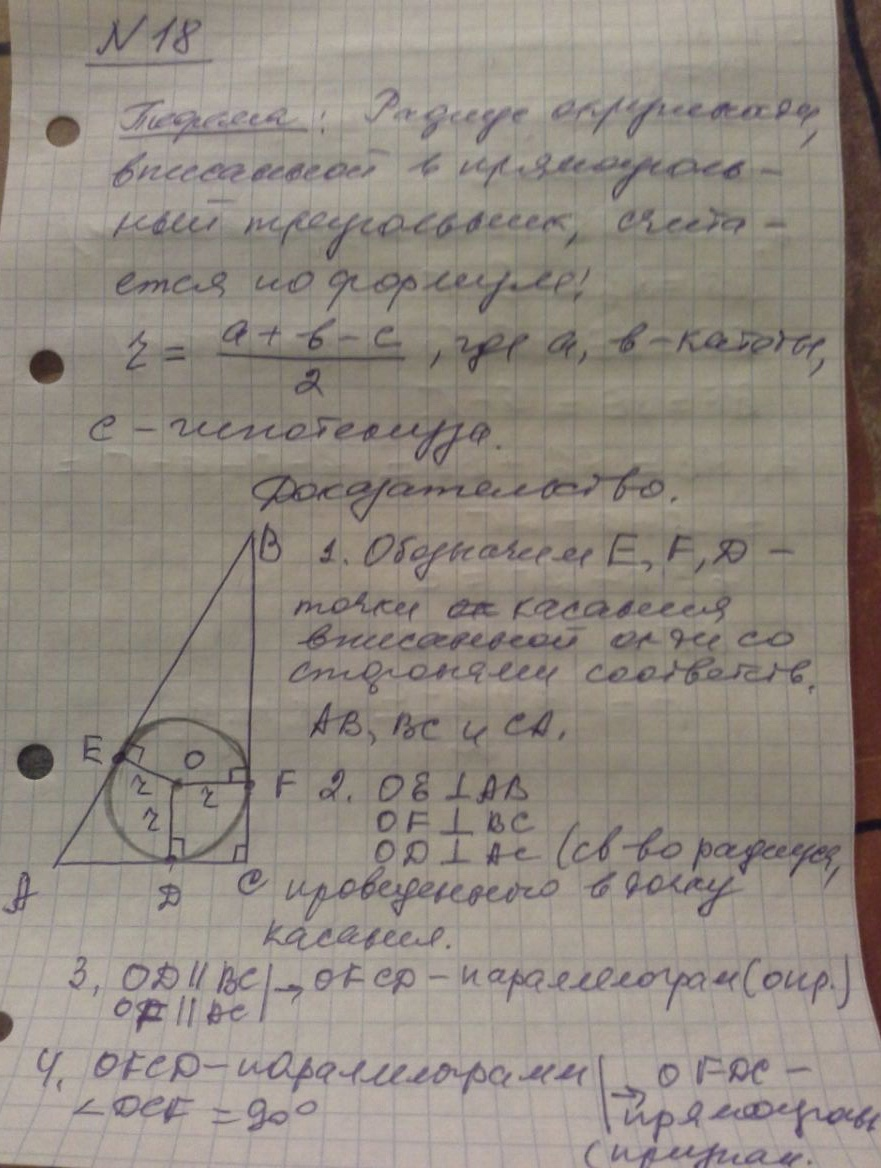
\includegraphics[scale=0.3]{solve18.jpg} \\
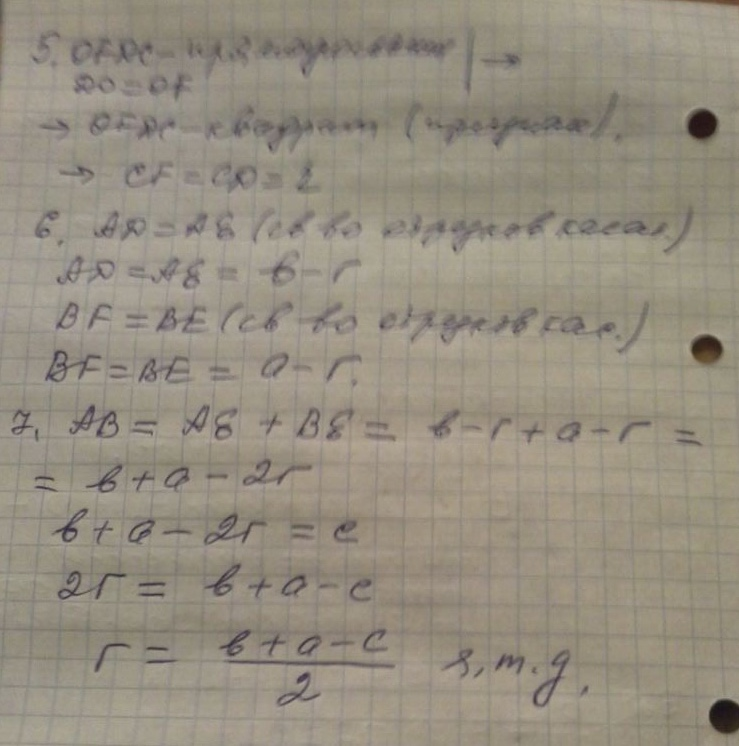
\includegraphics[scale=0.3]{solve18-2.jpg} \\
\section {Сформулируйте и докажите условия перпендикулярности и коллинеарность векторов через их координаты.} 

\end{document}